%Dies ist die Hauptseite des Dokumentes. Es werden u. a. alle Kapitel, Einstellung im Header eingebunden.
%Ver�nderungen m�ssen in folgenden Dateien vorgenommen werden:
			%- Layout.tex 
			%- newComments.tex
			%- Titelseite
			%- Versions�bersicht
			%- einzelne Kapitel (evtl. erweitern) 
			
% Definition von globalen Parametern, die derzeit auf der Titelseite und in der Kopfzeile 
% verwendet werden. Der in <> gesetzte Text ist zu ver�ndern.  

\newcommand{\praktikumTitel}{<Titel des Praktikums>}
\newcommand{\projektTitel}{<Titel des Teilprojektes>}


%Hier sind alle Einstellungen enthalten, die sich auf das Seiten- und Dokumentenlayout beziehen

\documentclass[
	11pt,								% Schriftgr��e
	DIV12,
	german,							% f�r Umlaute, Silbentrennung etc.
	oneside,						% einseitiges Dokument
	titlepage,					% es wird eine Titelseite verwendet
	halfparskip,				% Abstand zwischen Abs�tzen (halbe Zeile)
	normalheadings,			% Gr��e der �berschriften verkleinern
	tablecaptionabove,	% Beschriftung von Tabellen unterhalb ausgeben
	final								% Status des Dokuments (final/draft)
]{scrreprt}						% 


%------�ndern von Schriftschnitten - (Muss ganz am Anfang stehen !) -------------
\usepackage{fix-cm}

%------Umlaute ------------------------------------------------------------------
% 	Umlaute/Sonderzeichen wie ���� k�nnen direkt im Quelltext verwenden werden.
%		Erlaubt automatische Trennung von Worten mit Umlauten.
\usepackage[T1]{fontenc}								 
\usepackage[latin1]{inputenc}

%------Anpassung der Landessprache-----------------------------------------------
\usepackage{ngerman}

%------Einfache Definition der Zeilenabst�nde und Seitenr�nder-------------------
\usepackage{geometry}
\usepackage{setspace}
\usepackage{tocbasic}

%------Schriftgr��enanpassung von einzelnen Textpassagen-------------------------
\usepackage{relsize}

%------Trennlinien in Kopf- und Fusszeile
\usepackage[headsepline, footsepline, ilines]{scrpage2}

%------Grafiken------------------------------------------------------------------
\usepackage{graphicx}
\usepackage{float}

%------Packet zum Sperren, Unterstreichen und Hervorheben von Texten------------
\usepackage{soul}

%------erg�nzende Schriftart----------------------------------------------------
\usepackage{helvet}

%------Lange Tabellen-----------------------------------------------------------
\usepackage{longtable}
\usepackage{array}
\usepackage{ragged2e}
\usepackage{lscape}

\usepackage{xparse}
\usepackage{framed}
\usepackage[usenames,dvipsnames]{color}

%------PDF-Optionen-------------------------------------------------------------
\usepackage[
	bookmarks,
	bookmarksopen=true,
	colorlinks=true,
	linkcolor=black,				% einfache interne Verkn�pfungen
	anchorcolor=black,			% Ankertext
	citecolor=black, 				% Verweise auf Literaturverzeichniseintr�ge im Text
	filecolor=black, 				% Verkn�pfungen, die lokale Dateien �ffnen
	menucolor=black, 				% Acrobat-Men�punkte
	urlcolor=black, 				% Farbe f�r URL-Links
	backref,								% Zur�cktext nach jedem Bibliografie-Eintrag als Liste von �berschriftsnummern
	pagebackref,						% Zur�cktext nach jedem Bibliografie-Eintrag als Liste von Seitenzahlen
	plainpages=false,				% zur korrekten Erstellung der Bookmarks
	pdfpagelabels,					% zur korrekten Erstellung der Bookmarks
	hypertexnames=false,		% zur korrekten Erstellung der Bookmarks
	% linktocpage 						% Seitenzahlen anstatt Text im Inhaltsverzeichnis verlinken
	]{hyperref}



			% enth�lt eingebundene Packete

%------Seitenr�nder-------------------------------------------------------------
\geometry{verbose, 										% zeigt die eingestellten Parameter beim Latexlauf an
			paper=a4paper, 									% Papierformat			
			top=25mm, 											% Rand oben
			left=25mm, 											% Rand links
			right=25mm, 										% Rand rechts
			bottom=45mm, 										% Rand unten
			pdftex													% schreibt das Papierformat in dei Ausgabe damit Ausgabeprogramm Papiergr��e erkennt		
	} 
	
%Seitenlayout
\onehalfspace        % 1,5-facher Abstand  

%------Kopf- und Fu�zeilen ------------------------------------------------------
\pagestyle{scrheadings}

%------Kopf- und Fu�zeile auch auf Kapitelanfangsseiten -------------------------
\renewcommand*{\chapterpagestyle}{scrheadings}

%------Schriftform der Kopfzeile ------------------------------------------------
\renewcommand{\headfont}{\normalfont}

%------Kopfzeile-----------------------------------------------------------------
\setlength{\headheight}{21mm}				% H�he der Kopfzeile
\ihead{\large{\textsc{\praktikumTitel}}\\		% Text in der linken Box
			 \small{\projektTitel}}
\chead{}														% Text in der mittleren Box

%----Fusszeile
\cfoot{}														% Text in mittlerer Box
\ofoot{\pagemark}										% Seitenzahl in rechter Box			





					% Diese Datei enth�lt alle Layouteinstellungen

%------Beginn des Gesamtdokumentes--------------------------------------------------------
\usepackage[ngerman]{babel}
\usepackage{hyperref}
\begin{document}
\shorthandoff{"}
%------Eingebundene Seiten, Verzeichnisse bzw. Kapitel------------------------------------
%----Stil dieser Seite--------------------------------------------------------------------
\thispagestyle{plain}			% Kopfzeile bleibt leer

%----Beginn der Titelseite----------------------------------------------------------------
\begin{titlepage}

%----zentrierte Ausrichtung �ber die gesamte Seite----------------------------------------		
\begin{center}

%----Titel des Praktikum (\praktikumTitel in newComments zu ver�ndern)--------------------
{\relsize{4}{\textbf{\textsc{\praktikumTitel}}}}\\[5ex]

%----Titel des Teilprojektes (\projektTitel in newComments ver�ndern)---------------------
{\relsize{3}{\textbf{\textsc{\projektTitel}}}}\\[5ex]

Praxis der Softwarentwicklung\\
Sommersemester 2014\\[6ex]

{\relsize{3}\so{\textbf{Qualit�tssicherung}}}\\[5ex]

%----Titelbild------------------------------------------------------------

\includegraphics[scale=0.25]{bilder/logo.png}\\[5ex]

%----Daten des Auftraggebers
Auftraggeber\\[2ex]															
KIT - Karlsruher Institut f�r Technologie\\
Fakult�t f�r Informatik\\										
Institut f�r Anthropromatik und Robotik (IAR)\\
Intelligente Prozessautomation und Robotik (IPR)\\[2ex]
Betreuer: Andreas Bihlmaier\\
andreas.bihlmaier@gmx.net\\[5ex]

% ----Tabelle Teilnehmer---------------------------------------------------
Auftragnehmer\\

\begin{tabular}{l<{\hspace{20mm}} l<{\hspace{30mm}}}\\	
	Name 									& 	E-Mail-Adresse\\			% Zeilen�berschift
		
	\hline										% Linie unterhalb der Zeilen�berschrift
	
	%----Nachfolgend alle Namen und E-Mail-Adressen der Teilnehmer einf�gen	
	Alex Weber & alex.weber3@gmx.net\\
	Matthias Hadlich & matthias.hadlich@student.kit.edu\\
	Matthias Klatte	& matthias.klatte@go4more.de\\
	Micha Wetzel & micha.wetzel@student.kit.edu\\	
	Sebastian Kneipp &	sebastian.kneipp@gmx.net
	
	
\end{tabular}\\[2ex]

\end{center}

\vfill Karlsruhe, 22.09.2014

\end{titlepage}
											% Titelseite	
% %kp ob wir des brauchen

%----�berschrift------------------------------------------------------------
{\relsize{2}\textbf{Versions�bersicht}}\\[2ex] 	

%----Start der Tabelle------------------------------------------------------
\begin{longtable}{|m{1.78cm}|m{1.59cm}|m{2.86cm}|m{1.9cm}|m{5.25cm}|}

	\hline																							% Linie oberhalb	
	
	%----Spalten�berschriften------------------------------------------------
	\textbf{Version}	&		\textbf{Datum}	&		\textbf{Autor}	&		\textbf{Status}	&		\textbf{Kommentar}	\\	%Spalten�berschrift	
	\hline																							% Gitterlinie
	
	%----die nachfolgeden beiden Zeilen so oft wiederholen und die ... mit den entsprechenden Daten zu f�llen wie erforderlich
	...		&		...		&		...		&		...		&		...\\				% Eintrag in Zeile
	\hline																							% Gitterlinie unten
	
%----Ende der Tabelle------------------------------------------------------	
\end{longtable}

				% Versions�bersicht
\tableofcontents													% Inhaltsverzeichnis wird automatisch generiert
\newpage
% \listoffigures														% ebenso das Abbildungsverzeichnis					

%----Kapitel des Feinentwurfs, die mit Inhalt zu f�llen sind------------------------------

\chapter{Einleitung}

Das Robot Operating System (ROS) ist eine Middleware, um flexible Robotik
Software zu schreiben. 2007 begann Willow Garage mit der Entwicklung von ROS,
welches heute in der Robotik Community weit verbreitet ist.
Es liefert eine Sammlung von Tools, Libraries und Konventionen, welche das
Erstellen von komplexer und robuster Robotik Software auf verschiedenen
Platformen erleichtern soll.
ROS gliedert die Algorithmen zur Realisierung intelligenter Roboter in einzelne
Aufgaben, welche durch jeweils einen Prozess (Node) dargestellt und auf mehrere
Rechner (Hosts) verteilt sein k�nnen.
Die Nodes verbinden sich nach dem Publisher-Subscriber Schema �ber ein Netzwerk
miteinander, um die Datenfl�sse herzustellen (ROS Graph).

\begin{figure}[H] \centering 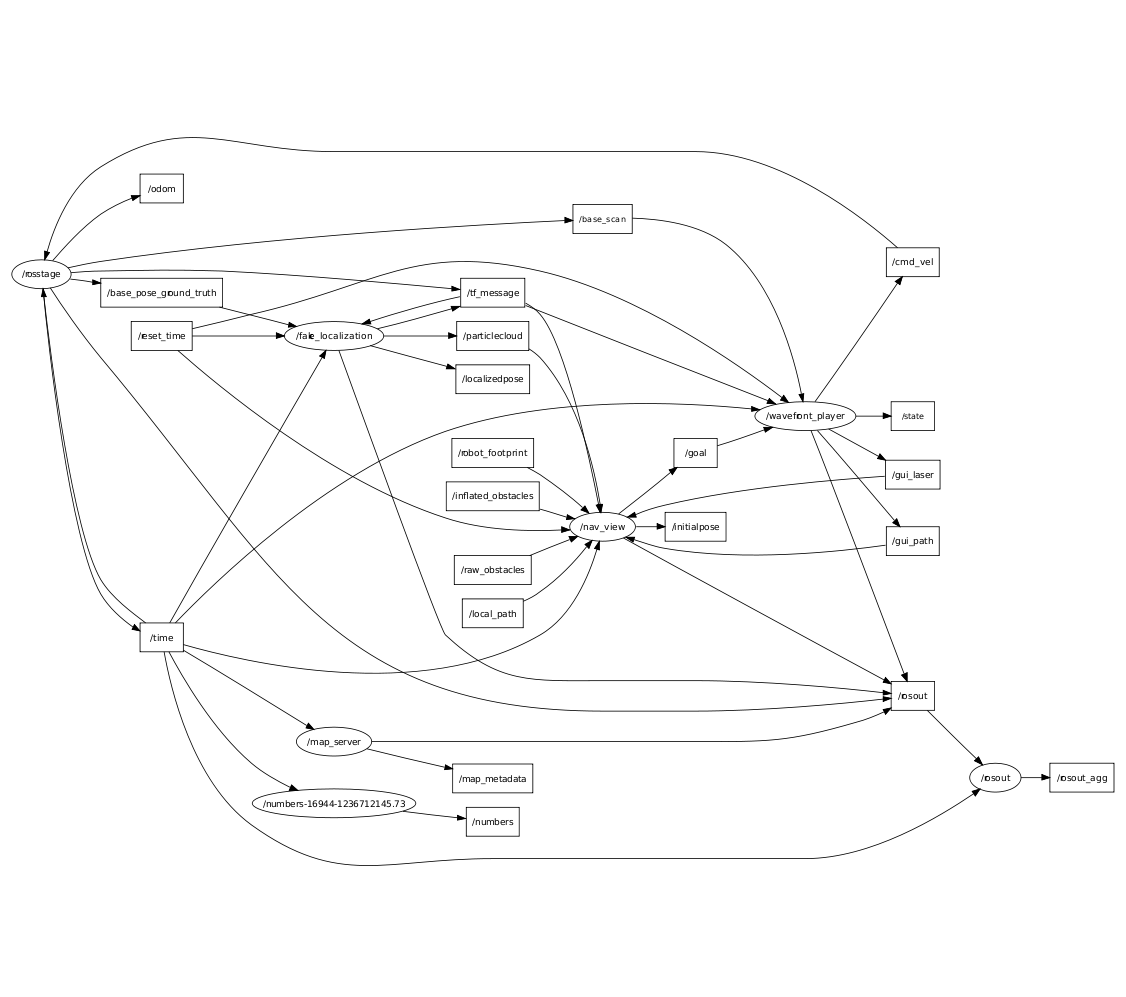
\includegraphics[scale=0.35]{./bilder/rxgraph.png}
\caption{Beispiel eines ROS Graph. Nodes sind als Ellipsen, Topics als Rechtecke
und Datenfluss als Pfeile dargestellt.
Quelle: http://www.willowgarage.com }
\end{figure}

Ein Problem stellt die �berwachung dieses Systems dar. Zwar besteht im Moment
die M�glichkeit, das Gesamtsystem auf Fehler zu �berpr�fen, jedoch ist es nicht
m�glich zu bestimmen, welcher Knoten sich fehlerhaft verh�lt. Dies kann
besonders bei gro�en System mit hunderten von Knoten zum Problem werden. Um ein
schnelles Debuggen zu erm�glichen, bedarf es einer Software zum dezentralen
Erfassen der Fehlerursachen.

Unser Ziel als PSE-Team ist es, ein System zur Definiton des Soll-Zustandes und
zum �berwachen des Ist-Zustandes individueller Knoten zu erstellen.

\NewDocumentEnvironment{unittest}{ m o }{
	\textbf{#1}\\
}{
	\begin{flushright}
		\IfNoValueTF {#2}
			{\colorbox{Red}{\textit{Fehlgeschlagen}}}
			{\colorbox{ForestGreen}{\textit{Bestanden}}}
	\end{flushright}
}

\chapter{Unittests}

\section{Arni\_Core}
\subsection*{TestSeuid}

\begin{unittest}{test\_valid\_noarg}[pass]
	Kein Argument ist keine g�ltige SEUID.
\end{unittest}
\begin{unittest}{test\_valid\_override}[pass]
	Die Methode is\_valid() funktioniert statisch auf einem g�ltigen SEUID Objekt.
\end{unittest}
\begin{unittest}{test\_valid\_from\_class}[pass]
	Erstellen eines SEUID Objektes mit ung�ltiger SEUID wirft einen NameError.\\
	Die Methode is\_valid() gibt auf einem g�ltig initialisiertem SEUID Objekt den richtigen Wert zur�ck.
\end{unittest}
\begin{unittest}{test\_valid\_from\_fn}[pass]
	Die Methode is\_valid() funktioniert statisch auf einem SEUID Objekt ohne eigene SEUID.
\end{unittest}
\begin{unittest}{test\_valid\_types}[pass]
	�berpr�ft verschiedene g�ltige und ung�ltige SEUIDs.
\end{unittest}
\begin{unittest}{test\_valid\_from\_serialization}[pass]
	Testet die Konstruktion mit einem serialisierten SEUID Objekt.
\end{unittest}
\begin{unittest}{test\_fields\_node}[pass]
	Testet, ob die �ffentlichen Attribute des Objektes mit einer Node-SEUID richtig gesetzt werden.
\end{unittest}
\begin{unittest}{test\_fields\_override}[pass]
	�berpr�ft, ob die �ffentlichen Attribute des Objektes zur�ckgesetzt werden, wenn es mit einem anderen Typ SEUID initialisiert wird.
\end{unittest}
\begin{unittest}{test\_fields\_connection}[pass]
	�berpr�ft die �ffentlichen Attribute eines Connection-SEUID Objektes.
\end{unittest}
\begin{unittest}{test\_msg\_invalid}[pass]
	Die Konstruktion mit einem Objekt, das kein g�ltiger Nachrichtentyp ist, wirft einen TypeError.
\end{unittest}
\begin{unittest}{test\_msg\_hostmsg}[pass]
	Testet die Konstruktion anhand einer HostMessage.
\end{unittest}
\begin{unittest}{test\_get\_seuid}[pass]
	Die Methode get\_seuid() liefert f�r eine SEUID falls vorhanden die SEUID des enthaltenen Hosts/Nodes/Publishers/Subscribers.
\end{unittest}
\begin{unittest}{test\_get\_seuid\_invalid}[pass]
	Die Methode get\_seuid() wirft einen AttributeError, wenn das Objekt nicht mit einer SEUID initalisiert wurde.\\
	Die Methode get\_seuid() wirft einen KeyError, wenn die angefragte SEUID nicht im Objekt vorhanden ist.
\end{unittest}

\section{Arni\_Processing}
\subsection*{TestLoadingSpecifications}

\begin{unittest}{test\_no\_specifications}[pass]
	Der Specificationhandler ist am Anfang leer, wenn er keine Spezifikationen im Namespace findet.
\end{unittest}
\begin{unittest}{test\_load\_spec}[pass]
	Testet, ob eine Spezifikation mit der angegebenen SEUID nach dem Laden vorhanden ist.\\
	Verwendet das format \texttt{[seuid1:{}]}.
\end{unittest}
\begin{unittest}{test\_load\_new\_specs}[pass]
	�berpr�ft, dass auch das format \texttt{section: [seuid1:{}]} geladen wird.
\end{unittest}
\begin{unittest}{test\_reload\_spec}[pass]
	�berpr�ft, dass Spezifikationen zu SEUIDs in den Bestand geladen wurden, nachdem sie auf den Parameterserver geladen und die reload-Methode aufgerufen wurde.
\end{unittest}
\begin{unittest}{test\_invalid\_seuid}[pass]
	�berpr�ft, dass keine Spezifikationen geladen werden, die keine gültige SEUID haben.
\end{unittest}
\begin{unittest}{test\_existing\_fields}[pass]
	�berpr�ft, alle Felder der Definition durch den Parameterserver gekommen sind und im Specification Objekt vorhanden sind.
\end{unittest}

\section{Arni\_Countermeasure}
\subsection*{Test parsing of constraints}

\begin{unittest}{test\_empty\_reaction}[pass]
    Simuliert eine leere reaction in einem constraint und erwartet das dies keine Exception verursacht.  
\end{unittest}

\begin{unittest}{test\_interval\_timeout\_not\_existing}[pass]
    Testet ob die standart Werte von min\_reaction\_interval und reaction\_timeout geladen werden wenn ein constraint diese nicht angibt.
\end{unittest}

\begin{unittest}{test\_interval\_valid\_values}[pass]
    Testet ob das setzen von min\_reaction\_interval und reaction\_timeout erfolgreich interpretiert werden.
\end{unittest}

\begin{unittest}{test\_interval\_wrong\_value}[pass]
    Testet ob bei invalider Eingabe f�r min\_reaction\_interval auf den standart Wert zur�ckgegriffen wird.
\end{unittest}

\begin{unittest}{test\_missing\_reactions}[pass]
    Simuliert fehlende reactions in einem constraint und erwartet das dies keine Exception verursacht.    
\end{unittest}

\begin{unittest}{test\_reaction\_autonomy\_level\_not\_set}[pass]
    Testet ob eine reaction welche kein autonomy level gesetzt hat erfolgreich interpretiert wird.
\end{unittest}

\begin{unittest}{test\_reaction\_multiple\_reactions}[pass]
    Testet ob zwei reactions in einem constraint als zwei reactions interpretiert werden.
\end{unittest}

\begin{unittest}{test\_reaction\_parse\_empty\_reaction}[pass]
    Testet ob eine leere reaction interpretiert weiterhin eine leere reaction ist.
\end{unittest}

\begin{unittest}{test\_reaction\_parse\_publish\_reaction}[pass]
    Testet ob eine publish reaction erfolgreich interpretiert wird.
\end{unittest}

\begin{unittest}{test\_reaction\_parse\_wrong\_action}[pass]
    Testet ob die Interpretation einer reaction mit falscher action eine leere reaction zur�ckgibt.
\end{unittest}

\begin{unittest}{test\_traverse\_empty\_and}[pass]
    Testet ob eine leere Und-Verkn�pfung erfolgreich interpretiert wird.
\end{unittest}

\begin{unittest}{test\_traverse\_simple\_and}[pass]
    Testet ob eine einfach Und-Verkn�pfung korrekt interpretiert wird.
\end{unittest}

\begin{unittest}{test\_traverse\_simple\_and\_or}[pass]
    Testet ob eine Or-Verkn�pfung in einer Und-Verkn�pfung korrekt interpretiert wird.
\end{unittest}

\begin{unittest}{test\_traverse\_simple\_not}[pass]
    Testet ob eine logische Invertierung korrekt interpretiert wird.
\end{unittest}

\begin{unittest}{test\_traverse\_wrong\_format}[pass]
    Testet ob eine Verkn�pfung bei der Interpretation ignoriert wird wenn sie von falschem Format ist.
\end{unittest}

\begin{unittest}{test\_traverse\_wrong\_outcome}[pass]
    Testet ob ein constraint Eintrag dessen Outcome kein String ist bei der interpretation ignoriert wird.
\end{unittest}



\subsection*{Test Reaction}

\begin{unittest}{test\_reaction\_restart}[pass]
    Testet ob die Aktion einen Knoten neuzustarten erfolgreich ausgef�hrt wird.
\end{unittest}


\begin{unittest}{test\_restart\_no\_host}[pass]
    Testet ob eine reaction eine korrekte Fehlermeldung ausgibt falls sie keinen Host zu dem Knoten, der neugestartet werden soll, findet.
\end{unittest}


\begin{unittest}{test\_restart\_no\_service}[pass]
    Testet ob eine reaction eine korrekte Fehlermeldung ausgibt falls der Service zum neustarten eines Knotens nicht verf�gbar ist.
\end{unittest}


\begin{unittest}{test\_run\_no\_host}[pass]
    Testet ob eine reaction eine korrekte Fehlermeldung ausgibt falls sie keinen Host zu dem Knoten, auf dessen Host ein Befehl ausgef�hrt werden soll, findet.
\end{unittest}


\begin{unittest}{test\_run\_no\_service}[pass]
    Testet ob eine reaction eine korrekte Fehlermeldung ausgibt falls der Service zum ausf�hren eines Befehls nicht verf�gbar ist.
\end{unittest}


\begin{unittest}{test\_shutdown\_no\_host}[pass]
    Testet ob eine reaction eine korrekte Fehlermeldung ausgibt falls sie keinen Host zu dem Knoten, der gestoppt werden soll, findet.
\end{unittest}


\begin{unittest}{test\_shutdown\_no\_service}[pass]
    Testet ob eine reaction eine korrekte Fehlermeldung ausgibt falls der Service zum stoppen eines Knotens nicht verf�gbar ist.
\end{unittest}




\subsection*{Test Scenario}


\begin{unittest}{test\_constraint\_timeout}[pass]
    Testet ob nach dem Ausf�hren einer Reaction solange zu n�chsten Ausf�hrung gewartet wird wie der Timeout ist.
\end{unittest}


\begin{unittest}{test\_high\_cpu}[pass]
    Testet ob eine Reaction in einem Constraint erfolgreich ausgef�hrt wird, wenn Outcome HIGH f�r cpu\_usage\_max �ber /statistics\_rated empfangen wird.
\end{unittest}


\begin{unittest}{test\_high\_cpu\_too\_short}[pass]
    Testet ob eine Reaction in einem Constraint nicht ausgef�hrt wird, wenn Outcome HIGH f�r cpu\_usage\_max �ber /statistics\_rated nicht lange genug empfangen wird.
\end{unittest}


\begin{unittest}{test\_reaction\_autonomy\_level\_too\_high}[pass]
    Testet ob eine Reaction in einem Constraint nicht ausgef�hrt wird, wenn das autonomy\_level zu hoch ist.
\end{unittest}




\subsection*{Test Storage}


\begin{unittest}{test\_add\_new\_than\_old}[pass]
    Testet ob eine zeitlich �ltere Statistik keine zeitlich neueren Statistiken �berschreibt. (Obwohl die �ltere sp�ter hinzugef�gt wird)
\end{unittest}


\begin{unittest}{test\_add\_old}[pass]
    Testet ob das hinzuf�gen einer zu alten Statistik verworfen wird.
\end{unittest}


\begin{unittest}{test\_callback\_multiple\_entries}[pass]
    Testet ob ein Aufruf mit einem bewerteten Statistik-Eintrag, welcher ein Array enth�lt, erfolgreich gespeichert wird.
\end{unittest}


\begin{unittest}{test\_callback\_multiple\_rated\_entities}[pass]
    Testet ob ein Aufruf mit mehreren bewerteten Statistik-Eintr�gen erfolgreich gespeichert wird.
\end{unittest}


\begin{unittest}{test\_callback\_single\_entry}[pass]
    Testet ob ein Aufruf mit einem bewerteten Statistik-Eintrag erfolgreich gespeichert wird.
\end{unittest}


\begin{unittest}{test\_remove\_through\_timeout}[pass]
    Testet ob eine hinzugef�gte Statistik nach dem Timeout nicht mehr vorhanden ist.
\end{unittest}


\section{Arni\_Nodeinterface}
\subsection*{Test Service}

\begin{unittest}{test\_kill}[pass]
	Testen den Service um einen Node zu stoppen, erwartet das erfolgreiche stoppen des Nodes
\end{unittest}

\begin{unittest}{test\_restart}[pass]
	Testet das neustarten eines Nodes. Erwartet den erfolgreichen Neustart
\end{unittest}

\subsection{Test statistical Calc}

\begin{unittest}{test\_cpu}[pass]
	Testet ob die statistischen Gr��en bei gegebenen Werten richtig berechnet werden.
\end{unittest}

\begin{unittest}{test\_cpu\_core}[pass]
	Testet ob die statistischen Gr��en bei Listen von Listen richtig berechnet werden.
\end{unittest}

\begin{unittest}{test\_empty\_list}[pass]
	Testet ob bei einer leeren Listen 0 - werte ausgegeben werden.
\end{unittest}
	


\chapter{Integrationstests}

\section{Test 1 - Gleichm��iges Publizieren }
Dieser Test pr�ft, ob bei stetigem Publizieren die Frequenz korrekt bewertet wird und ob auf die Bewertung korrekt reagiert wird.

\begin{enumerate}
    \item Test-Launchfile starten:
    Mit \texttt{roslaunch arni\_core test\_1\_steady.launch} wird das Launchfile gestartet.\\
    Man sieht, dass dabei folgende Knoten gestartet werden:
    \begin{verbatim}
        countermeasure (arni_countermeasure/arni_countermeasure)
        ninja_turtle (arni_core/predefined_subscriber.py)
        node_manager (arni_nodeinterface/arni_nodeinterface)
        processing (arni_processing/arni_processing)
        steady_tree (arni_core/predefined_publisher.py)
    \end{verbatim}
    Debei besteht folgende Verbindung der Knoten (Debugging-Knoten zur �bersichtlichkeit ausgenommen):\\

\begin{figure}[htbp]
    \begin{minipage}[t]{16cm}
        \vspace{0pt}
        \centering
        
\includegraphics[scale=0.3]{./bilder/integrationstests/test_1_nodegraph.png}
        \caption{steady\_tree publiziert mit 100Hz auf /forest, ninja\_turtle abonniert forest.}
    \end{minipage}
    \hfill
\end{figure}  

    Die Frequenz von /forest wird unter 80Hz als LOW und �ber 120Hz als HIGH bewertet.
    Der Countermeasure-Knoten hat das Constraint alle 10 Sekunden \textit{frequency of forest is ok} auszugeben, falls die Frequenz mit OK bewertet wurde.

\newpage
    \item �ffnen der GUI:
    In die Konsole wird \texttt{rosrun rqt\_gui rqt\_gui} eingegeben und ausgef�hrt.\\
    \item �ffnen der Widgets:
    Ausw�hlen des Widgets \textit{Logging > Console},\\
    Debug Messages ausblenden\\

\begin{figure}[htbp]
    \begin{minipage}[t]{16cm}
        \vspace{0pt}
        \centering
        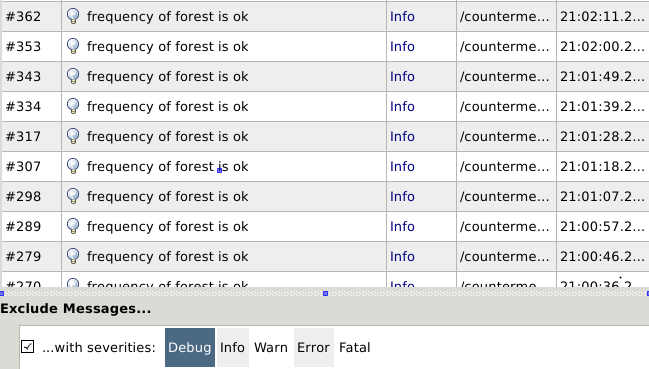
\includegraphics[scale=0.5]{./bilder/integrationstests/test_1_rqt_freq_ok.png}
        \caption{steady\_tree publiziert mit 100Hz auf forest. ninja\_turtle h�rt zu.}
    \end{minipage}
    \hfill
\end{figure}  


    Es ist zu sehen, dass die Nachricht des Countermeasure-Knotens alle 10 Sekunden publiziert wird.
\end{enumerate}


\newpage
\section{Test 2 - Zu niedrige Frequenz }
Dieser Test pr�ft das Verhalten beim Publizieren mit geringerer Frequenz als durch die Spezifikationen erwartet wird und ob auf die Bewertung korrekt reagiert wird.

\begin{enumerate}
    \item Test-Launchfile starten:
    Mit \texttt{roslaunch arni\_core test\_2\_steady\_low.launch} wird das Launchfile gestartet.\\
    Man sieht, dass dabei folgende Knoten gestartet werden:
    \begin{verbatim}
        countermeasure (arni_countermeasure/arni_countermeasure)
        leopard_seal (arni_core/predefined_subscriber.py)
        node_manager (arni_nodeinterface/arni_nodeinterface)
        processing (arni_processing/arni_processing)
        breathing_penguin (arni_core/predefined_publisher.py)
    \end{verbatim}
    Debei besteht folgende Verbindung der Knoten (Debugging-Knoten zur �bersichtlichkeit ausgenommen):\\

\begin{figure}[htbp]
    \begin{minipage}[t]{16cm}
        \vspace{0pt}
        \centering
        
\includegraphics[scale=0.3]{./bilder/integrationstests/test_2_nodegraph.png}
        \caption{breathing\_penguin publiziert mit 200Hz auf /antarctica, leopard\_seal abonniert antarctica.}
    \end{minipage}
    \hfill
\end{figure}  

    Die Frequenz von /antarctica wird unter 400Hz als LOW und �ber 600Hz als HIGH bewertet.
    Der Countermeasure-Knoten hat das Constraint alle 5 Sekunden \textit{frequency of antarctica is too low} auszugeben, falls die Frequenz mit LOW bewertet wurde.

\newpage
    \item �ffnen der GUI:
    In die Konsole wird \texttt{rosrun rqt\_gui rqt\_gui} eingegeben und ausgef�hrt.\\
    \item �ffnen der Widgets:
    Ausw�hlen des Widgets \textit{Logging > Console},\\
    Debug Messages ausblenden\\

\begin{figure}[htbp]
    \begin{minipage}[t]{16cm}
        \vspace{0pt}
        \centering
        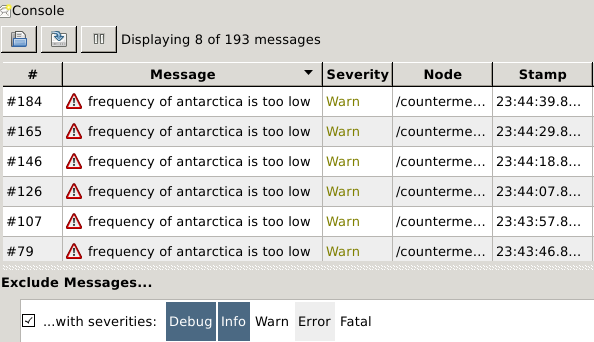
\includegraphics[scale=0.5]{./bilder/integrationstests/test_2_log.png}
        \caption{breathing\_penguin publiziert mit 200Hz auf /antarctica. leopard\_seal h�rt zu.}
    \end{minipage}
    \hfill
\end{figure}  


    Es ist zu sehen, dass die Nachricht des Countermeasure-Knotens alle 5 Sekunden publiziert wird.
\end{enumerate}


\newpage
\section{Test 3 - Variierende Frequenz }
Dieser Test pr�ft das Verhalten beim Publizieren mit variierender Frequenz in einer Sinuskurve, wobei hohe Werte als zu hoch und niedrige Werte als zu niedrig bewertet werden.

\begin{enumerate}
	\item Test-Launchfile starten:
	Mit \texttt{roslaunch arni\_core test\_3\_fluctuation.launch} wird das Launchfile gestartet.\\
	Man sieht, dass dabei folgende Knoten gestartet werden:
	\begin{verbatim}
	    countermeasure (arni_countermeasure/arni_countermeasure)
	    sailing_boat (arni_core/predefined_subscriber.py)
	    node_manager (arni_nodeinterface/arni_nodeinterface)
	    processing (arni_processing/arni_processing)
	    fluctuation_tide (arni_core/predefined_publisher.py)
	\end{verbatim}
	Debei besteht folgende Verbindung der Knoten (Debugging-Knoten zur �bersichtlichkeit ausgenommen):\\

\begin{figure}[htbp]
    \begin{minipage}[t]{16cm}
        \vspace{0pt}
        \centering
        
\includegraphics[scale=0.3]{./bilder/integrationstests/test_3_nodegraph.png}
        \caption{fluctuation\_tide publiziert mit einer Frequenz zwischen 10 und 190 auf /ocean, sailing\_boat abonniert ocean.}
    \end{minipage}
    \hfill
\end{figure}  

    Die Frequenz von /ocean wird unter 70Hz als LOW und �ber 130Hz als HIGH bewertet.
    Unterschreitet die aufgezeichnete Frequenz die Grenze, wird \textit{frequency of ocean is too low} auszugeben, \textit{frequency of ocean is too high}, wenn die Frequenz 130Hz �berschreitet und \textit{frequency of ocean is ok} sonst.

\newpage
	\item �ffnen der GUI:
	In die Konsole wird \texttt{rosrun rqt\_gui rqt\_gui} eingegeben und ausgef�hrt.\\
	\item �ffnen der Widgets:
	Ausw�hlen des Widgets \textit{Logging > Console},\\
    Debug Messages ausblenden\\

\begin{figure}[htbp]
    \begin{minipage}[t]{16cm}
        \vspace{0pt}
        \centering
        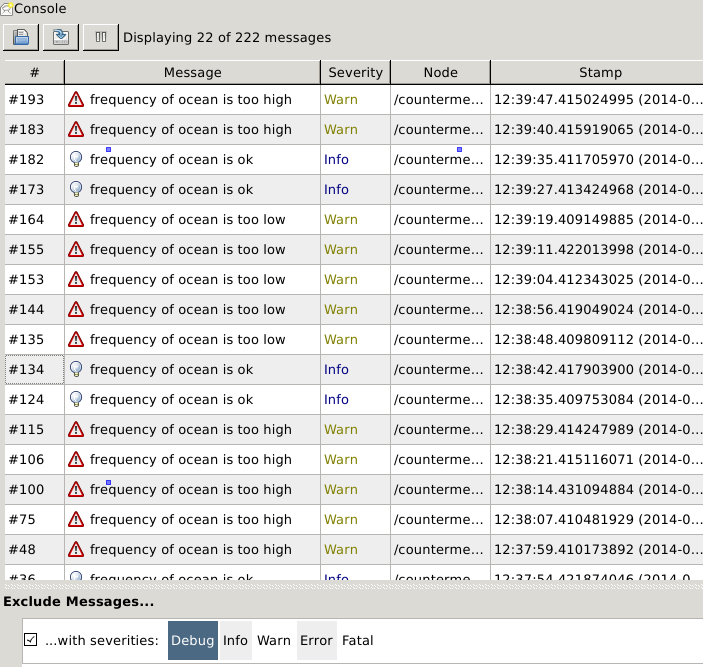
\includegraphics[scale=0.5]{./bilder/integrationstests/test_3_log.png}
        \caption{fluctuation\_tide publiziert mit 10 - 190Hz auf /ocean. sailing\_boat h�rt zu.}
    \end{minipage}
    \hfill
\end{figure}  


    Es ist zu sehen, dass sich \textit{[...] is ok}, \textit{[...] is too high}, \textit{[...] is ok}, \textit{[...] is too low}, etc. abwechseln.
\end{enumerate}

\chapter{Code-Abdeckung}
Da sich die Code-Abdeckung unter ROS nur sehr bedingt testen l�sst, konnten nur die nachfolgenden Ergebnisse gesammelt werden. Automatische Tests konnten nicht analysiert werden, sodass die Datenerhebung lediglich durch Probieren von Testszenarien stattfinden konnte, was in einigen Bereichen die von Unittests abgedeckten Abschnitte nicht vollst�ndig erreicht.
\\
Die Daten wurden mit dem Tool \textit{coverage.py}\footnote{\label{foot:1}Coverage l�sst sich �ber \texttt{pip install coverage} installieren.} in den n�her beschriebenen Szenarien erhoben. Dazu wurde das Start-Script der Knoten ausgef�hrt und abschlie�end der Report auf die relevanten Dateien gek�rzt.

\section{Nodeinterface}

\begin{figure}[htbp]
    \begin{minipage}[t]{16cm}
        \vspace{0pt}
        \centering
        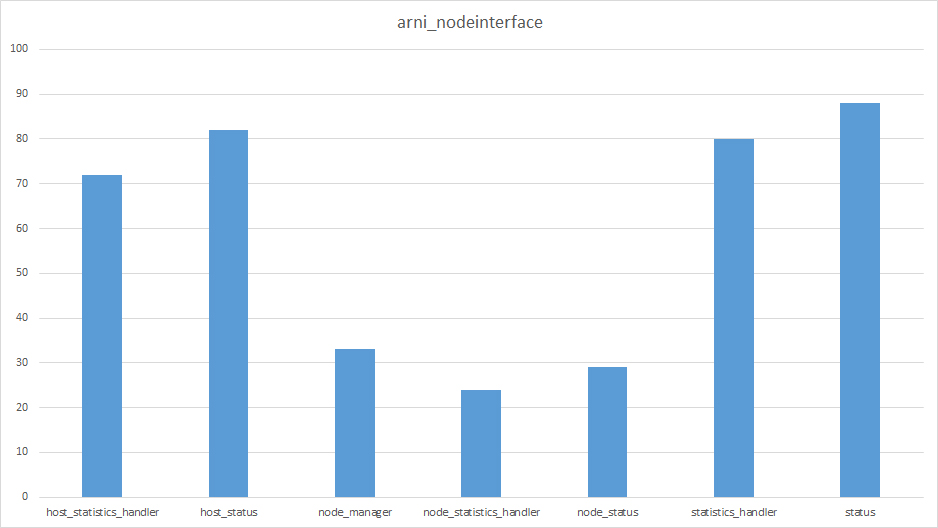
\includegraphics[scale=0.5]{./bilder/coverage/coverage_nodeinterface.jpg}
        \caption{Die dargestellten Daten wurden im Normalbetrieb des Nodeinterface Knotens erhoben, wobei �u�ere Zugriffe auf die Services nicht dargestellt werden konnten, weshalb entsprechende Bereiche unterrepr�sentiert sind.}
    \end{minipage}
    \hfill
\end{figure}  

\newpage
\section{Processing}

\begin{figure}[htbp]
    \begin{minipage}[t]{16cm}
        \vspace{0pt}
        \centering
        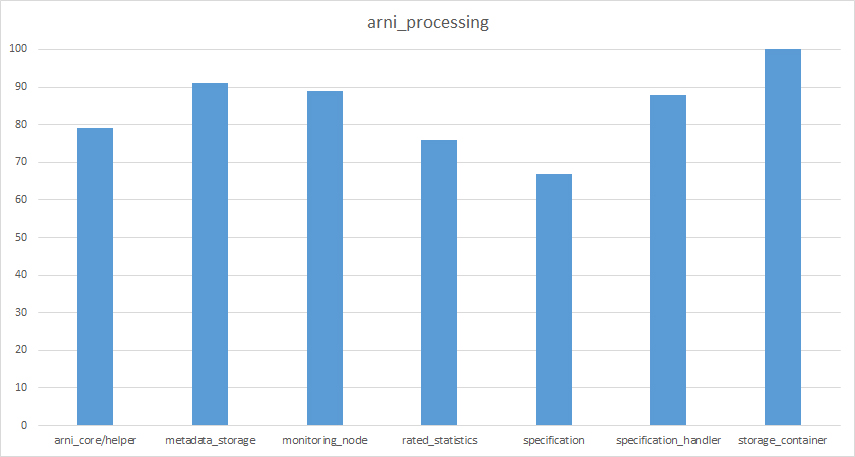
\includegraphics[scale=0.5]{./bilder/coverage/coverage_processing.jpg}
        \caption{Zur Erhebung der dargestellten Daten liefen mehrere Knoten (arni\_core/tutorial\_*) und ein Nodeinterface. Nachtr�glich wurde die GUI gestartet, die sich Daten �ber einen Service holte. Au�erdem wurden verz�gert Spezifikationen geladen, die auch einen Service bnuzten. Nach einer Weile wurde ein Knoten abgeschaltet, woraufhin Nachrichten �ber seine Fehlfunktion gesendet wurden.}
    \end{minipage}
    \hfill
\end{figure}  

\newpage
\section{Countermeasure}

\begin{figure}[htbp]
    \begin{minipage}[t]{16cm}
        \vspace{0pt}
        \centering
        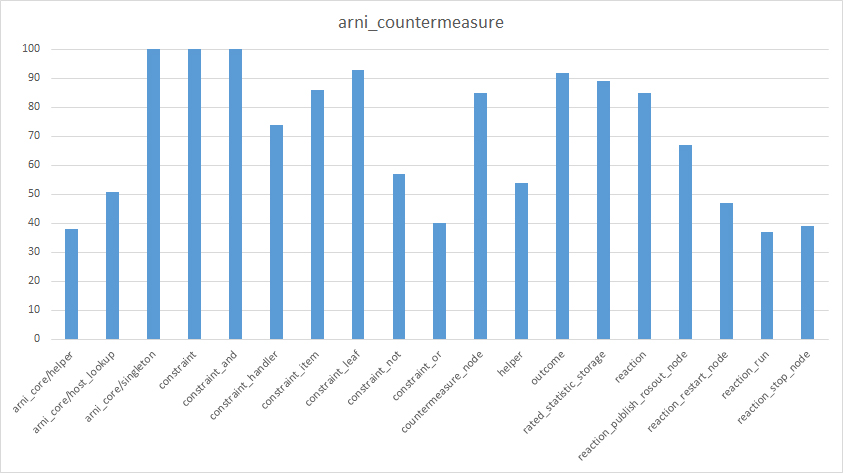
\includegraphics[scale=0.55]{./bilder/coverage/coverage_countermeasure4.jpg}
        \caption{Die dargestellten Werte wurden erreicht, indem Integrationstest 4 durchgef�hrt wurde.}
    \end{minipage}
    \hfill
\end{figure}  

\newpage
\section{GUI}

\begin{figure}[htbp]
    \begin{minipage}[t]{16cm}
        \vspace{0pt}
        \centering
        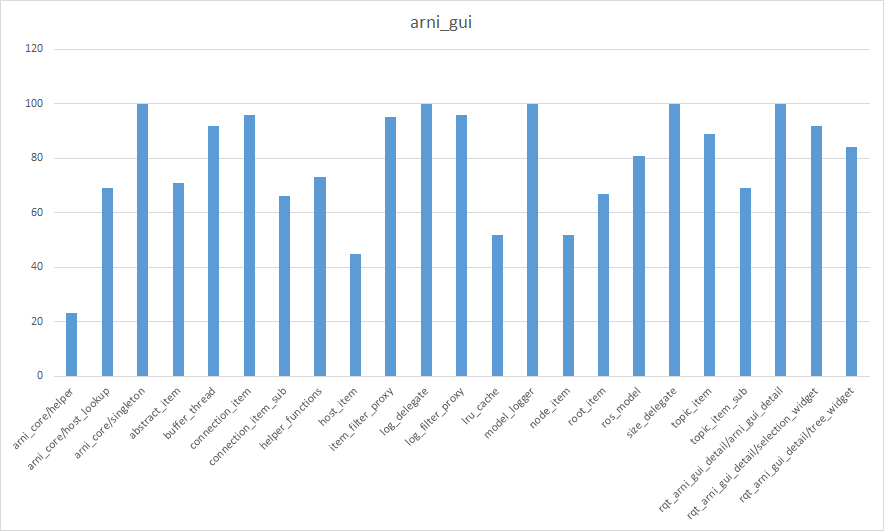
\includegraphics[scale=0.55]{./bilder/coverage/coverage_gui.jpg}
        \caption{Die dargestellten Werte wurden erreicht, indem Integrationstest 4 und Arni-Detail betrachtet wurde. Dabei wurden strukturiert alle Features der �bersichtsliste durchgegangen, beinhaltend Filter und Ansichtsoptionen. Anschlie�end wurden verschiedene Itemtypen ausgew�hlt. Die einzelnen Tabs der Detailanzeige wurden ge�ffnet und verf�gbare Steuerelemente benutzt.}
    \end{minipage}
    \hfill
\end{figure}  
				

%------Ende des Dokumentes----------------------------------------------------------------
\end{document}
